\subsection{Большие мультимодальные модели}
Большие мультимодальные модели (\texttt{Large Multimodal Model}, \texttt{LMM}) способны обрабатывать разные входные данные, например видео, аудио, изображение. Способность обрабатывать информацию из разных данных делают эту модель некоторым расширением возможностей классических языковых моделей (\texttt{LLM}). В общем смысле, \texttt{LMM} представляют собой комбинацию \texttt{LLM} и унифицированных под каждый тип данных энкодеров, например свёрточные нейронные сети для изображений, трансформеры для текстов, спектрограммы для аудио. Затем происходит операция связывания (\texttt{fusion}), что обеспечивает взаимодействие между признаками разных модальностей, а также даёт возможность составлять комбинированные функции потерь.

В контексте курсовой работы, \texttt{LMM} применяется для генерации подробных и структурированных описаний одежды и позы человека на входном изображении, которые в дальнейшем можно использовать, например, в латентных диффузионных моделях (\texttt{Latent Diffusion Model}, \texttt{LDM}). Операция применения выходов одной модели для запуска другой модели называется стэкинг (\texttt{stacking}). После перечисления аттрибутов позы и одежды, выбираются $n^{\{p, c\}}$ наиболее информативных признаков: $A^{\{p, c\}} = \{a_1^{\{p, c\}}, \dots, a_{n^{\{p, c\}}}^{\{p, c\}}\}$. В зависимости от условий, можно контроллировать процесс отбора признаков. Так, в силу ограниченности длины лексем в кодировщике \texttt{CLIP}, стоит выбирать более глобальные признаки, такие как материал, цвет. Используя описания вместо \texttt{DensePose}, удаётся сохранить архитектуру \texttt{text"=to"=image} \cite{promptdresser}.

При входном изображении $x \in \{x^p, x^c\}$ и \texttt{LMM} $\mathcal{M}$, предсказанные описания $\mathcal{K}^{\{p, c\}}$ можно получить следующим образом:
\begin{gather}
    \mathcal{K}^{\{p, c\}} = \{k_1^{\{p, c\}}, \dots, k_{n^{\{p, c\}}}^{\{p, c\}}\} = \mathcal{M}(x|\mathcal{P}, \mathcal{D}_{ex}^{\{p, c\}}, \mathcal{T}^{\{p, c\}}),
\end{gather}
где $\mathcal{P}$ есть входной промпт, $\mathcal{D}_{ex}^{\{p, c\}}$ "--- набор данных для обучения в контексте, и $\mathcal{T}^{\{p, c\}}$ "--- описание задачи. Процесс генерации маски на основе текстового запроса можно увидеть на изображении \ref{fig:lmm_maskgener} \cite{promptdresser}.

\begin{figure}[H]
    \centering
    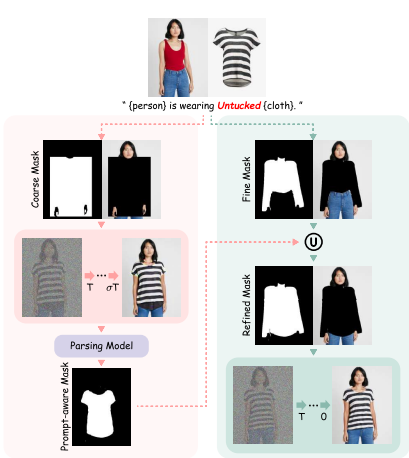
\includegraphics[width=0.75\linewidth]{images/lmm_maskgener.png}
    \caption{Процесс генерации маски с помощью \texttt{LMM}}
    \label{fig:lmm_maskgener}
\end{figure}

Основным преимуществом \texttt{LMM} является универсальность, поскольку модель может работать с несколькими модальностями. Помимо этого, для задач виртуальной примерочной полезно связывать изображение с его текстовым описанием, с чем мультимодальная модель очень хорошо справляется, а обучение на разнотипных данных даёт устойчивость к качеству исходных изображений, что позволяет генерировать более стабильные результаты. К недостаткам данной модели можно отнести факт того, что без тщательной фильтрации \texttt{LMM} может включать в промпты упоминания старой одежды, что приводит к артефактам и некорректному редактированию изображения. Помимо этого, точность и полнота промптов зависит от выбранной \texttt{LMM} (\texttt{GPT"=4o}, \texttt{LLaVA} и др.), что может привести к нестабильным результатом при смене модели. Помимо этого, мультимодальная модель может не так точно передавать более мелкие признаки, такие как узор одежды, крой, материал, что может снизить итоговое качество.

\subsubsection{Использование \texttt{LMM}}
Метод \texttt{PromptDresser} ориентируется на создание виртуальной примерочной, которая будет регулироваться посредством текстовых запросов. Так, задача сводится к генерации изображения $x^p$ на основе изображения $x^c$ с помощью методов обработки текста, предоставляемых в \texttt{LMM}. Общий подход к решению данной задачи можно рассмотреть на изображении \ref{fig:prompt_pipeline} \cite{promptdresser}.

Подход \texttt{PromptDresser} основывается на \texttt{LDM}, который состоит из трёх основных компонент: \texttt{VAE} с кодировщиком $\mathcal{E}(\cdot)$ и декодировщиком $\mathcal{G}(\cdot)$, текстовый кодировщик $\tau(\cdot)$ и основная \texttt{UNet} $\epsilon_0$. Предобученный \texttt{VAE} кодирует исходное изображение $x$ в в латентное пространство меньшей размерности: $z_0 = \mathcal{E}(x)$. Затем происходит восстановление в $\texttt{RGB}$ посредством декодировщика: $\hat{x} = \mathcal{G}(z_0)$. \texttt{UNet} предобучена для предсказания значения $z_0$ на основе $z_t$, где 
\begin{gather}
    z_t = \mathcal{N}(z_t; \sqrt{\overline{\alpha}}z_0, (1 - \overline{\alpha_t})I)
\end{gather}
Функция потерь \texttt{LDM} выглядит следующим образом:
\begin{gather}
    \mathcal{L}_{LDM} = \mathbb{E}_{z_0 \sim \mathcal{E}(x), \epsilon \sim \mathcal{N}(0, I), y, t}[||\epsilon - \epsilon_0 (z_t, t, \tau(y)||_2^2]
\end{gather}
Данная функция нацелена на уменьшение разницы между получившимся шумом $\epsilon$, и шумом, предсказанным с помощью \texttt{UNet}.
\begin{figure}[H]
    \centering
    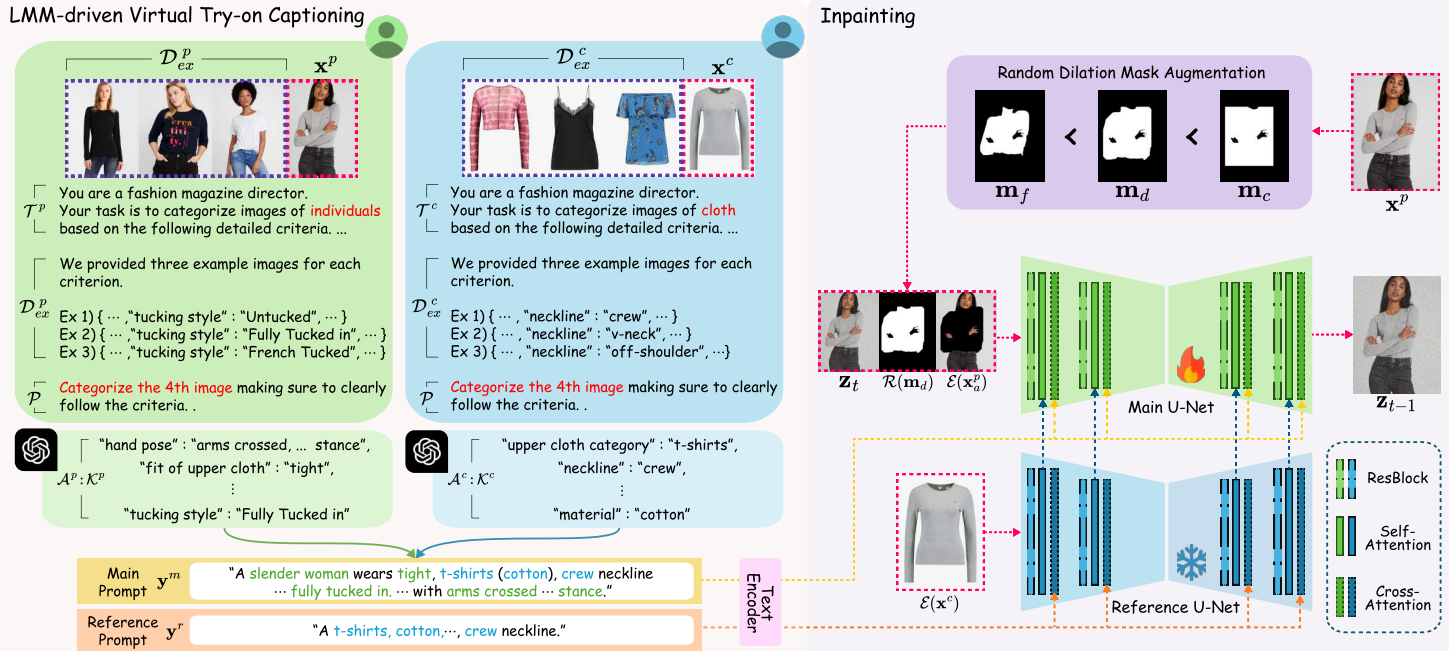
\includegraphics[width=0.95\linewidth]{images/prompt_pipeline.png}
    \caption{Подход \texttt{PromptDresser} в решении задачи \texttt{VITON}}
    \label{fig:prompt_pipeline}
\end{figure}
Далее, с помощью \texttt{GPT"=4o} происходит генерация текстовых подсказок, что позволяет разделить описание позы и описание одежды. Вводится метод генерации масок от грубых (\texttt{coarse}) к тонким (\texttt{fine}), что позволяет адаптивно выбирать область редактирования, обеспечивая баланс между качеством и контролем \cite{promptdresser}. Для грубой маски $m_c$ и тонкой маски $m_f$, расширенная маска $m_d$, используемая в обучении, может быть получена следующим образом:
\begin{gather}
    m_d = (m_f \oplus^n b) \cap m_c,
\end{gather}
где $\oplus^n$ означает операцию обобщения со структурным элементов $b$ $n$ раз.